% Options for packages loaded elsewhere
\PassOptionsToPackage{unicode}{hyperref}
\PassOptionsToPackage{hyphens}{url}
%
\documentclass[
]{article}
\usepackage{lmodern}
\usepackage{amssymb,amsmath}
\usepackage{ifxetex,ifluatex}
\ifnum 0\ifxetex 1\fi\ifluatex 1\fi=0 % if pdftex
  \usepackage[T1]{fontenc}
  \usepackage[utf8]{inputenc}
  \usepackage{textcomp} % provide euro and other symbols
\else % if luatex or xetex
  \usepackage{unicode-math}
  \defaultfontfeatures{Scale=MatchLowercase}
  \defaultfontfeatures[\rmfamily]{Ligatures=TeX,Scale=1}
\fi
% Use upquote if available, for straight quotes in verbatim environments
\IfFileExists{upquote.sty}{\usepackage{upquote}}{}
\IfFileExists{microtype.sty}{% use microtype if available
  \usepackage[]{microtype}
  \UseMicrotypeSet[protrusion]{basicmath} % disable protrusion for tt fonts
}{}
\makeatletter
\@ifundefined{KOMAClassName}{% if non-KOMA class
  \IfFileExists{parskip.sty}{%
    \usepackage{parskip}
  }{% else
    \setlength{\parindent}{0pt}
    \setlength{\parskip}{6pt plus 2pt minus 1pt}}
}{% if KOMA class
  \KOMAoptions{parskip=half}}
\makeatother
\usepackage{xcolor}
\IfFileExists{xurl.sty}{\usepackage{xurl}}{} % add URL line breaks if available
\IfFileExists{bookmark.sty}{\usepackage{bookmark}}{\usepackage{hyperref}}
\hypersetup{
  pdftitle={Aprendizaje no supervisado: Árboles de desición},
  pdfauthor={Daniela Arbeláez Montoya; Jefferson Gamboa Betancur},
  hidelinks,
  pdfcreator={LaTeX via pandoc}}
\urlstyle{same} % disable monospaced font for URLs
\usepackage[margin=1in]{geometry}
\usepackage{color}
\usepackage{fancyvrb}
\newcommand{\VerbBar}{|}
\newcommand{\VERB}{\Verb[commandchars=\\\{\}]}
\DefineVerbatimEnvironment{Highlighting}{Verbatim}{commandchars=\\\{\}}
% Add ',fontsize=\small' for more characters per line
\usepackage{framed}
\definecolor{shadecolor}{RGB}{248,248,248}
\newenvironment{Shaded}{\begin{snugshade}}{\end{snugshade}}
\newcommand{\AlertTok}[1]{\textcolor[rgb]{0.94,0.16,0.16}{#1}}
\newcommand{\AnnotationTok}[1]{\textcolor[rgb]{0.56,0.35,0.01}{\textbf{\textit{#1}}}}
\newcommand{\AttributeTok}[1]{\textcolor[rgb]{0.77,0.63,0.00}{#1}}
\newcommand{\BaseNTok}[1]{\textcolor[rgb]{0.00,0.00,0.81}{#1}}
\newcommand{\BuiltInTok}[1]{#1}
\newcommand{\CharTok}[1]{\textcolor[rgb]{0.31,0.60,0.02}{#1}}
\newcommand{\CommentTok}[1]{\textcolor[rgb]{0.56,0.35,0.01}{\textit{#1}}}
\newcommand{\CommentVarTok}[1]{\textcolor[rgb]{0.56,0.35,0.01}{\textbf{\textit{#1}}}}
\newcommand{\ConstantTok}[1]{\textcolor[rgb]{0.00,0.00,0.00}{#1}}
\newcommand{\ControlFlowTok}[1]{\textcolor[rgb]{0.13,0.29,0.53}{\textbf{#1}}}
\newcommand{\DataTypeTok}[1]{\textcolor[rgb]{0.13,0.29,0.53}{#1}}
\newcommand{\DecValTok}[1]{\textcolor[rgb]{0.00,0.00,0.81}{#1}}
\newcommand{\DocumentationTok}[1]{\textcolor[rgb]{0.56,0.35,0.01}{\textbf{\textit{#1}}}}
\newcommand{\ErrorTok}[1]{\textcolor[rgb]{0.64,0.00,0.00}{\textbf{#1}}}
\newcommand{\ExtensionTok}[1]{#1}
\newcommand{\FloatTok}[1]{\textcolor[rgb]{0.00,0.00,0.81}{#1}}
\newcommand{\FunctionTok}[1]{\textcolor[rgb]{0.00,0.00,0.00}{#1}}
\newcommand{\ImportTok}[1]{#1}
\newcommand{\InformationTok}[1]{\textcolor[rgb]{0.56,0.35,0.01}{\textbf{\textit{#1}}}}
\newcommand{\KeywordTok}[1]{\textcolor[rgb]{0.13,0.29,0.53}{\textbf{#1}}}
\newcommand{\NormalTok}[1]{#1}
\newcommand{\OperatorTok}[1]{\textcolor[rgb]{0.81,0.36,0.00}{\textbf{#1}}}
\newcommand{\OtherTok}[1]{\textcolor[rgb]{0.56,0.35,0.01}{#1}}
\newcommand{\PreprocessorTok}[1]{\textcolor[rgb]{0.56,0.35,0.01}{\textit{#1}}}
\newcommand{\RegionMarkerTok}[1]{#1}
\newcommand{\SpecialCharTok}[1]{\textcolor[rgb]{0.00,0.00,0.00}{#1}}
\newcommand{\SpecialStringTok}[1]{\textcolor[rgb]{0.31,0.60,0.02}{#1}}
\newcommand{\StringTok}[1]{\textcolor[rgb]{0.31,0.60,0.02}{#1}}
\newcommand{\VariableTok}[1]{\textcolor[rgb]{0.00,0.00,0.00}{#1}}
\newcommand{\VerbatimStringTok}[1]{\textcolor[rgb]{0.31,0.60,0.02}{#1}}
\newcommand{\WarningTok}[1]{\textcolor[rgb]{0.56,0.35,0.01}{\textbf{\textit{#1}}}}
\usepackage{graphicx,grffile}
\makeatletter
\def\maxwidth{\ifdim\Gin@nat@width>\linewidth\linewidth\else\Gin@nat@width\fi}
\def\maxheight{\ifdim\Gin@nat@height>\textheight\textheight\else\Gin@nat@height\fi}
\makeatother
% Scale images if necessary, so that they will not overflow the page
% margins by default, and it is still possible to overwrite the defaults
% using explicit options in \includegraphics[width, height, ...]{}
\setkeys{Gin}{width=\maxwidth,height=\maxheight,keepaspectratio}
% Set default figure placement to htbp
\makeatletter
\def\fps@figure{htbp}
\makeatother
\setlength{\emergencystretch}{3em} % prevent overfull lines
\providecommand{\tightlist}{%
  \setlength{\itemsep}{0pt}\setlength{\parskip}{0pt}}
\setcounter{secnumdepth}{-\maxdimen} % remove section numbering
\usepackage{booktabs}
\usepackage{longtable}
\usepackage{array}
\usepackage{multirow}
\usepackage{wrapfig}
\usepackage{float}
\usepackage{colortbl}
\usepackage{pdflscape}
\usepackage{tabu}
\usepackage{threeparttable}
\usepackage{threeparttablex}
\usepackage[normalem]{ulem}
\usepackage{makecell}
\usepackage{xcolor}

\title{Aprendizaje no supervisado: Árboles de desición}
\author{Daniela Arbeláez Montoya \and Jefferson Gamboa Betancur}
\date{}

\begin{document}
\maketitle

\begin{center}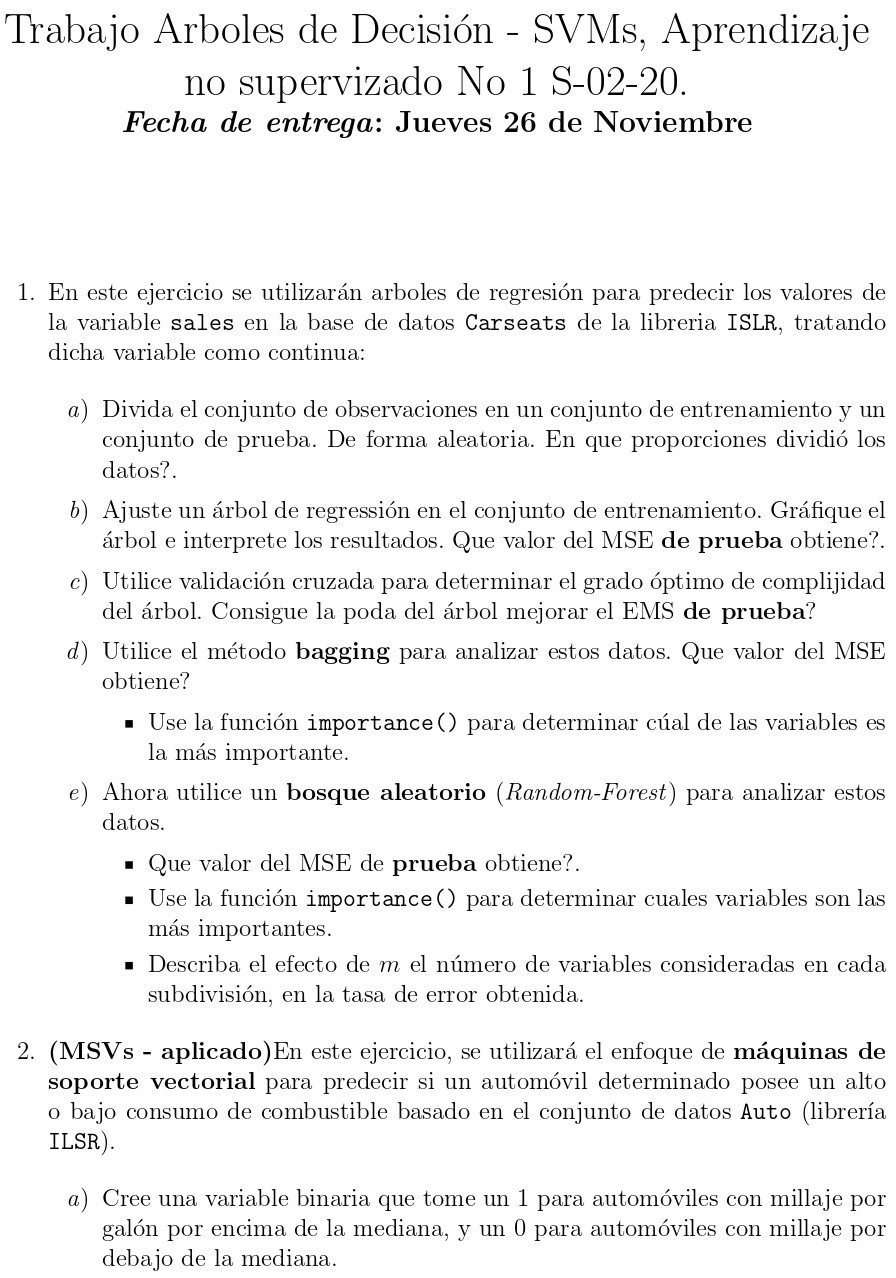
\includegraphics[width=0.8\linewidth]{Trabajo1_Mod3_Sem0220_page-0001} \end{center}

\begin{center}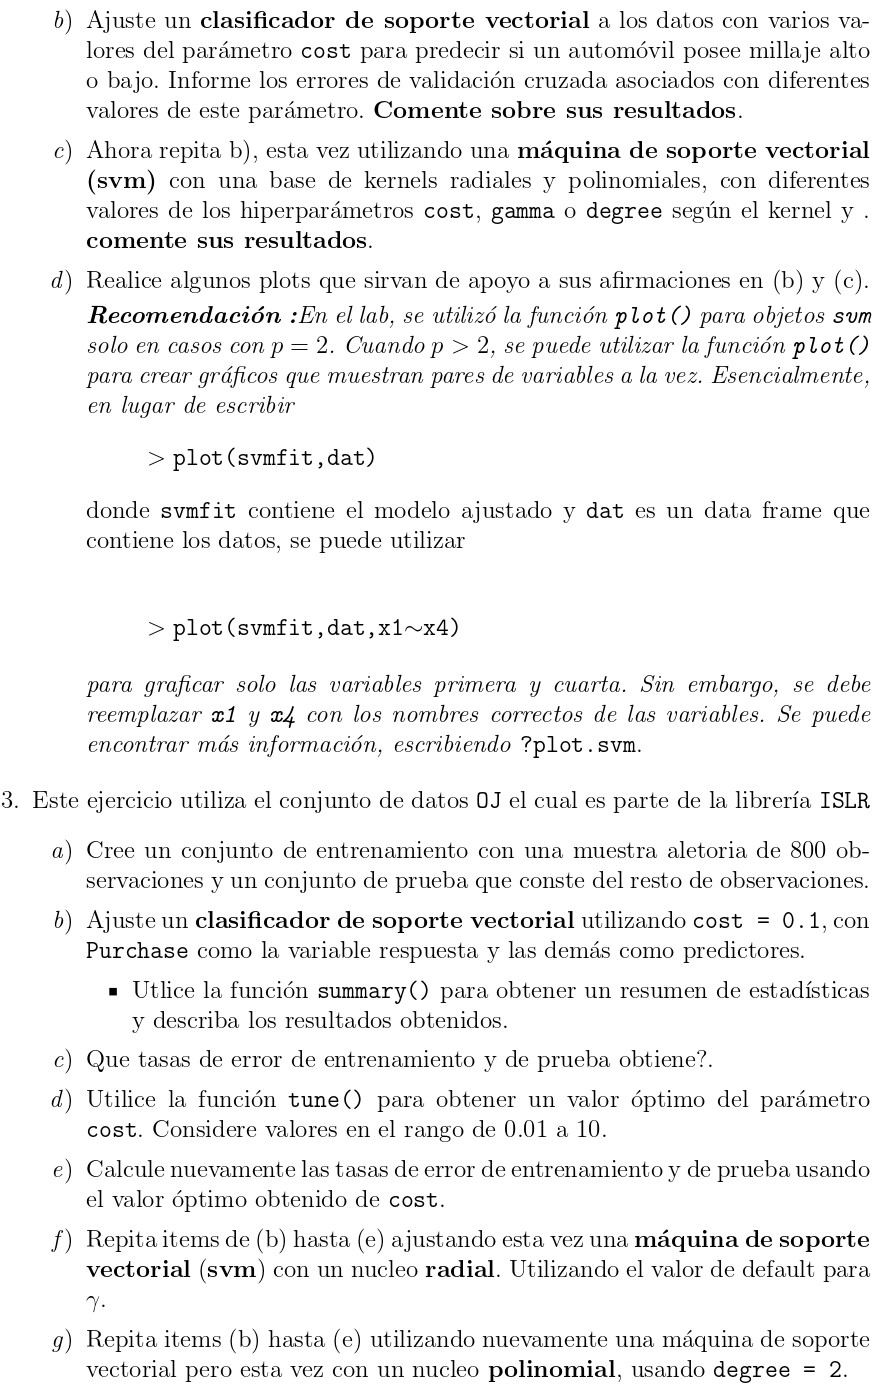
\includegraphics[width=0.9\linewidth]{Trabajo1_Mod3_Sem0220_page-0002} \end{center}

\begin{center}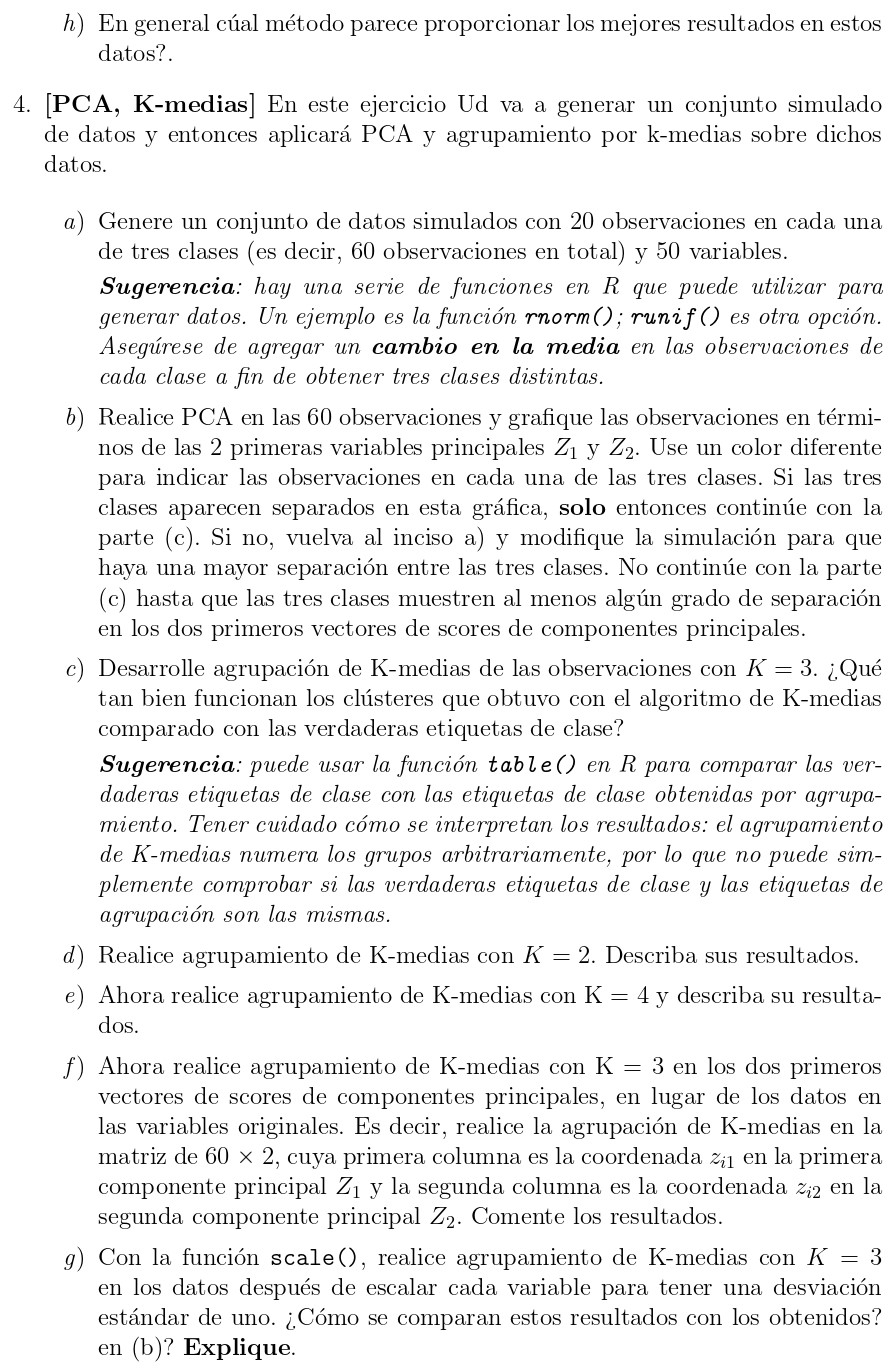
\includegraphics[width=0.9\linewidth]{Trabajo1_Mod3_Sem0220_page-0003} \end{center}

\begin{center}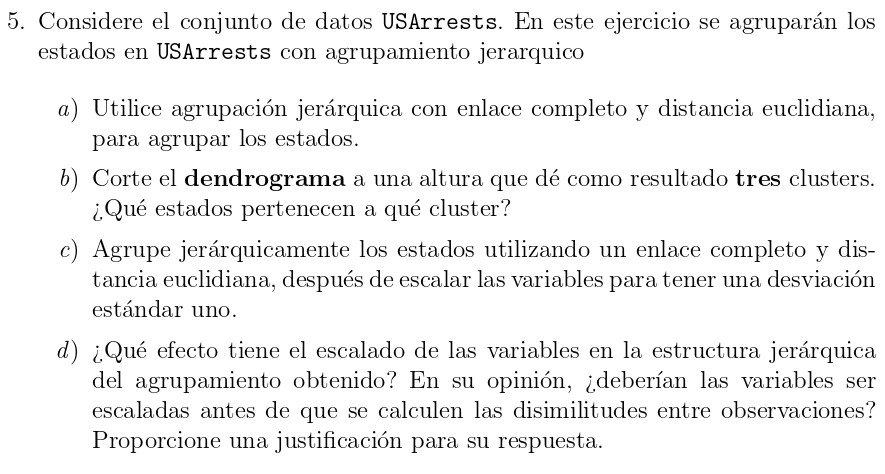
\includegraphics[width=0.9\linewidth]{Trabajo1_Mod3_Sem0220_page-0004} \end{center}

\hypertarget{soluciuxf3n}{%
\section{Solución}\label{soluciuxf3n}}

\begin{Shaded}
\begin{Highlighting}[]
\KeywordTok{require}\NormalTok{(ISLR)}
\NormalTok{datos <-}\StringTok{ }\NormalTok{Carseats}
\end{Highlighting}
\end{Shaded}

\textbf{Descripción de Carseats.}

Un conjunto de datos simulados que contiene las ventas de asientos de
seguridad para niños en 400 tiendas diferentes.

\textbf{Formato} Un marco de datos con 400 observaciones sobre las
siguientes 11 variables.

\textbf{Descripción de las variables}

\emph{Sales} Ventas unitarias (en miles) en cada ubicación

\emph{CompPrice} Precio cobrado por la competencia en cada ubicación

\emph{Income} Nivel de ingresos de la comunidad (en miles de dólares)

\emph{Advertising} Presupuesto de publicidad local para la empresa en
cada ubicación (en miles de dólares)

\emph{Population} Tamaño de la población en la región (en miles)

\emph{Price} Precio que cobra la empresa por los asientos de seguridad
en cada sitio

\emph{ShelveLoc} Un factor con niveles Malo, Bueno y Medio que indica la
calidad de la ubicación de las estanterías para los asientos del
automóvil en cada sitio.

\emph{Age} Edad media de la población local

\emph{Education} Nivel de educación en cada ubicación

\emph{Urban} Un factor con niveles No y Sí para indicar si la tienda
está en una ubicación urbana o rural.

\emph{US} Un factor con niveles No y Sí para indicar si la tienda está
en EE. UU. O no

\hypertarget{a}{%
\subsection{1.a)}\label{a}}

Los datos son particionados aleatoriamente en el 70\% para entrenamiento
(train) y el 30\% de prueba (test)

\begin{Shaded}
\begin{Highlighting}[]
\KeywordTok{set.seed}\NormalTok{(}\DecValTok{123}\NormalTok{)}
\NormalTok{muestra <-}\StringTok{ }\KeywordTok{sample}\NormalTok{(}\DecValTok{1}\OperatorTok{:}\KeywordTok{nrow}\NormalTok{(datos), }\DataTypeTok{size =} \KeywordTok{floor}\NormalTok{(}\KeywordTok{nrow}\NormalTok{(datos) }\OperatorTok{*}\StringTok{ }\FloatTok{0.7}\NormalTok{))}
\NormalTok{train <-}\StringTok{ }\NormalTok{datos[muestra, ]; test <-}\StringTok{ }\NormalTok{datos[}\OperatorTok{-}\NormalTok{muestra, ]}
\end{Highlighting}
\end{Shaded}

\hypertarget{b}{%
\subsection{1.b)}\label{b}}

\begin{Shaded}
\begin{Highlighting}[]
\KeywordTok{require}\NormalTok{(tree)}
\KeywordTok{require}\NormalTok{(MASS)}

\NormalTok{Reg.tree <-}\StringTok{ }\KeywordTok{tree}\NormalTok{(Sales }\OperatorTok{~}\StringTok{ }\NormalTok{., }\DataTypeTok{data =}\NormalTok{ datos, }\DataTypeTok{subset =}\NormalTok{ muestra)}
\KeywordTok{summary}\NormalTok{(Reg.tree)}
\end{Highlighting}
\end{Shaded}

\begin{verbatim}
## 
## Regression tree:
## tree(formula = Sales ~ ., data = datos, subset = muestra)
## Variables actually used in tree construction:
## [1] "ShelveLoc"   "Price"       "CompPrice"   "Age"         "Advertising"
## Number of terminal nodes:  19 
## Residual mean deviance:  2.373 = 619.2 / 261 
## Distribution of residuals:
##    Min. 1st Qu.  Median    Mean 3rd Qu.    Max. 
## -4.1570 -1.0160  0.1123  0.0000  0.8903  4.0310
\end{verbatim}

\begin{Shaded}
\begin{Highlighting}[]
\KeywordTok{plot}\NormalTok{(Reg.tree)}
\KeywordTok{text}\NormalTok{(Reg.tree, }\DataTypeTok{pretty =} \DecValTok{0}\NormalTok{)}
\end{Highlighting}
\end{Shaded}

\begin{center}\includegraphics[width=0.6\linewidth]{Tarea_files/figure-latex/unnamed-chunk-7-1} \end{center}

Observe que el árbol de regresión consideró que las variables más
importantes fueron:

\emph{ShelveLoc:} Un factor con niveles Malo, Bueno y Medio que indica
la calidad de la ubicación de las estanterías para los asientos del
automóvil en cada sitio.

\emph{Price:} Precio que cobra la empresa por los asientos de seguridad
en cada sitio.

\emph{CompPrice:} Precio cobrado por la competencia en cada ubicación.

\emph{Age:} Edad media de la población local.

\emph{Advertising:} Presupuesto de publicidad local para la empresa en
cada ubicación (en miles de dólares)

La calidad de la ubicación en las estanterías para los asientos es la
covariable más importante para determinar la venta unitaria en cada
ubicación, donde el la venta promedio del asiento es más baja cuando la
calidad del asiento esta entre baja y media, mientras que la venta
promedio para la calidad del asiento cuando es alta crece.

\begin{Shaded}
\begin{Highlighting}[]
\NormalTok{MSE1 <-}\StringTok{ }\KeywordTok{mean}\NormalTok{((test}\OperatorTok{$}\NormalTok{Sales }\OperatorTok{-}\StringTok{ }\KeywordTok{predict}\NormalTok{(Reg.tree, }\DataTypeTok{newdata =}\NormalTok{ test))}\OperatorTok{^}\DecValTok{2}\NormalTok{)}
\end{Highlighting}
\end{Shaded}

Y el MSE de prueba es de 3.602818

\hypertarget{c}{%
\subsection{1.c)}\label{c}}

Ahora se utilizará cv.tree para ver si una poda mejora su desempeño

\begin{Shaded}
\begin{Highlighting}[]
\KeywordTok{set.seed}\NormalTok{(}\DecValTok{123}\NormalTok{)}
\NormalTok{cv_Reg <-}\StringTok{ }\KeywordTok{cv.tree}\NormalTok{(Reg.tree)}
\NormalTok{D.prueba <-}\StringTok{ }\KeywordTok{data.frame}\NormalTok{(cv_Reg}\OperatorTok{$}\NormalTok{size, cv_Reg}\OperatorTok{$}\NormalTok{dev)}
\NormalTok{D.prueba <-}\StringTok{ }\NormalTok{D.prueba[}\KeywordTok{which.min}\NormalTok{(D.prueba[,}\DecValTok{2}\NormalTok{]),]}
\KeywordTok{plot}\NormalTok{(cv_Reg}\OperatorTok{$}\NormalTok{size, cv_Reg}\OperatorTok{$}\NormalTok{dev, }\DataTypeTok{type =} \StringTok{"b"}\NormalTok{, }\DataTypeTok{xlab =} \StringTok{"Tree seze"}\NormalTok{, }\DataTypeTok{ylab =} \StringTok{"MSE de validación cruzada"}\NormalTok{)}
\KeywordTok{points}\NormalTok{(D.prueba[,}\DecValTok{1}\NormalTok{],D.prueba[,}\DecValTok{2}\NormalTok{], }\DataTypeTok{pch=}\DecValTok{19}\NormalTok{, }\DataTypeTok{cex=}\DecValTok{2}\NormalTok{, }\DataTypeTok{col=}\StringTok{"red"}\NormalTok{)}
\KeywordTok{legend}\NormalTok{(}\StringTok{"topright"}\NormalTok{, }\DataTypeTok{inset =} \FloatTok{.05}\NormalTok{, }\DataTypeTok{legend=}\KeywordTok{c}\NormalTok{(}\StringTok{"size = 8"}\NormalTok{, }\StringTok{"mín MSE = 1300.186"}\NormalTok{), }\DataTypeTok{cex=}\FloatTok{0.8}\NormalTok{, }\DataTypeTok{box.lty=}\DecValTok{0}\NormalTok{)}
\end{Highlighting}
\end{Shaded}

\begin{center}\includegraphics[width=0.6\linewidth]{Tarea_files/figure-latex/unnamed-chunk-9-1} \end{center}

Luego se procede a realizar la poda con la funsión de R, prune.tree

\begin{Shaded}
\begin{Highlighting}[]
\NormalTok{prune.Reg <-}\StringTok{ }\KeywordTok{prune.tree}\NormalTok{(Reg.tree, }\DataTypeTok{best =} \DecValTok{8}\NormalTok{)}
\KeywordTok{plot}\NormalTok{(prune.Reg)}
\KeywordTok{text}\NormalTok{(prune.Reg, }\DataTypeTok{pretty =} \DecValTok{0}\NormalTok{)}
\end{Highlighting}
\end{Shaded}

\begin{center}\includegraphics[width=0.6\linewidth]{Tarea_files/figure-latex/unnamed-chunk-10-1} \end{center}

\begin{Shaded}
\begin{Highlighting}[]
\NormalTok{MSE2 <-}\StringTok{ }\KeywordTok{mean}\NormalTok{((test}\OperatorTok{$}\NormalTok{Sales }\OperatorTok{-}\StringTok{ }\KeywordTok{predict}\NormalTok{(prune.Reg, }\DataTypeTok{newdata =}\NormalTok{ test))}\OperatorTok{^}\DecValTok{2}\NormalTok{);}
\end{Highlighting}
\end{Shaded}

\begin{table}[H]
\centering
\begin{tabular}{cc}
\toprule
MSE sin poda & MSE con poda\\
\midrule
3.602818 & 4.353022\\
\bottomrule
\end{tabular}
\end{table}

Como se logra detallar el MSE de prueba sin poda es mucho menor al MSE
de prueba con poda, es decir que no podar el árbol con 8 nodos no ayuda
a mejorar el modelo.

\hypertarget{d}{%
\subsection{1.d)}\label{d}}

\begin{Shaded}
\begin{Highlighting}[]
\KeywordTok{require}\NormalTok{(randomForest)}
\KeywordTok{set.seed}\NormalTok{(}\DecValTok{123}\NormalTok{)}

\NormalTok{bas.Reg <-}\StringTok{ }\KeywordTok{randomForest}\NormalTok{(Sales }\OperatorTok{~}\StringTok{ }\NormalTok{. , }\DataTypeTok{data =}\NormalTok{ datos, }\DataTypeTok{subset =}\NormalTok{ muestra, }\DataTypeTok{mtry =} \DecValTok{10}\NormalTok{, }\DataTypeTok{importance =} \OtherTok{TRUE}\NormalTok{)}
\KeywordTok{importance}\NormalTok{(bas.Reg)}
\end{Highlighting}
\end{Shaded}

\begin{verbatim}
##                %IncMSE IncNodePurity
## CompPrice   34.4262904    257.760843
## Income       7.4645949    113.727916
## Advertising 20.4003141    147.788939
## Population  -3.0115418     66.776729
## Price       64.3523306    630.500603
## ShelveLoc   72.8822146    689.811838
## Age         17.7747876    182.686692
## Education    3.4693027     63.408518
## Urban       -0.8360222      8.755624
## US           0.2868891      8.107184
\end{verbatim}

\begin{Shaded}
\begin{Highlighting}[]
\KeywordTok{varImpPlot}\NormalTok{(bas.Reg)}
\end{Highlighting}
\end{Shaded}

\begin{center}\includegraphics[width=0.6\linewidth]{Tarea_files/figure-latex/unnamed-chunk-13-1} \end{center}

\begin{Shaded}
\begin{Highlighting}[]
\NormalTok{MSE3 <-}\StringTok{ }\KeywordTok{mean}\NormalTok{((test}\OperatorTok{$}\NormalTok{Sales }\OperatorTok{-}\StringTok{ }\KeywordTok{predict}\NormalTok{(bas.Reg, }\DataTypeTok{newdata =}\NormalTok{ test))}\OperatorTok{^}\DecValTok{2}\NormalTok{)}
\end{Highlighting}
\end{Shaded}

Las covariables \emph{ShelveLoc} y \emph{Price} son las covariables con
mayor importancia en la base de datos. El MSE de prueba que se obtuvo
utilizando bagging fue de 2.2817104

\hypertarget{e}{%
\subsection{1.e)}\label{e}}

Para bosques aleatorios se utilizará por defecto en mtry = p/3 para
generar el bosque.

\begin{Shaded}
\begin{Highlighting}[]
\KeywordTok{set.seed}\NormalTok{(}\DecValTok{123}\NormalTok{)}
\NormalTok{rf.Reg <-}\StringTok{ }\KeywordTok{randomForest}\NormalTok{(Sales }\OperatorTok{~}\StringTok{ }\NormalTok{. , }\DataTypeTok{data =}\NormalTok{ datos, }\DataTypeTok{subset =}\NormalTok{ muestra, }\DataTypeTok{importance =} \OtherTok{TRUE}\NormalTok{)}
\NormalTok{MSE4 <-}\StringTok{ }\KeywordTok{mean}\NormalTok{((test}\OperatorTok{$}\NormalTok{Sales }\OperatorTok{-}\StringTok{ }\KeywordTok{predict}\NormalTok{(rf.Reg, }\DataTypeTok{newdata =}\NormalTok{ test))}\OperatorTok{^}\DecValTok{2}\NormalTok{)}
\end{Highlighting}
\end{Shaded}

El MSE de prueba para random forest es de 2.6254673

\begin{Shaded}
\begin{Highlighting}[]
\KeywordTok{importance}\NormalTok{(rf.Reg)}
\end{Highlighting}
\end{Shaded}

\begin{verbatim}
##               %IncMSE IncNodePurity
## CompPrice   19.669545     224.50086
## Income       6.424047     163.98134
## Advertising 14.712752     183.97789
## Population   1.513814     122.15101
## Price       40.239965     501.07261
## ShelveLoc   50.020107     529.44556
## Age         17.817908     253.67201
## Education    1.881294     100.14106
## Urban        1.118754      19.28070
## US           4.085561      23.08111
\end{verbatim}

\begin{Shaded}
\begin{Highlighting}[]
\KeywordTok{varImpPlot}\NormalTok{(rf.Reg)}
\end{Highlighting}
\end{Shaded}

\begin{center}\includegraphics[width=0.6\linewidth]{Tarea_files/figure-latex/unnamed-chunk-15-1} \end{center}

Para random forest se encuentra que las mismas dos covariables que se
presentaron en bagging son las más importante.

Si se compara el MSE de prueba para el bagging y el de random forest es:

\begin{Shaded}
\begin{Highlighting}[]
\NormalTok{M <-}\StringTok{ }\KeywordTok{data.frame}\NormalTok{(MSE3, MSE4)}
\KeywordTok{names}\NormalTok{(M) <-}\StringTok{ }\KeywordTok{c}\NormalTok{(}\StringTok{"MSE bagging"}\NormalTok{, }\StringTok{"MSE random forest"}\NormalTok{)}

\KeywordTok{kable}\NormalTok{(}
\NormalTok{  M,}
  \DataTypeTok{align =} \StringTok{"c"}\NormalTok{,}
  \DataTypeTok{booktabs =} \OtherTok{TRUE}
\NormalTok{) }\OperatorTok\StringTok{ }\KeywordTok{kable_styling}\NormalTok{(}\DataTypeTok{position =} \StringTok{"center"}\NormalTok{)}
\end{Highlighting}
\end{Shaded}

\begin{table}[H]
\centering
\begin{tabular}{cc}
\toprule
MSE bagging & MSE random forest\\
\midrule
2.28171 & 2.625467\\
\bottomrule
\end{tabular}
\end{table}

Se observa que a pesar de utilizar con bagging un m = 10 y para random
forest un m = 10/3 se logra evidenciar el MSE de prueba del bagging es
mucho más pequeño que el de random forest, esto es devido a que random
forest tiene una presición mucho más baja que el otro método utilizado.

\hypertarget{a-1}{%
\subsection{2.a)}\label{a-1}}

\hypertarget{b-1}{%
\subsection{2.b)}\label{b-1}}

\hypertarget{c-1}{%
\subsection{2.c)}\label{c-1}}

\hypertarget{d-1}{%
\subsection{2.d)}\label{d-1}}

\hypertarget{a-2}{%
\subsection{3.a)}\label{a-2}}

\hypertarget{b-2}{%
\subsection{3.b)}\label{b-2}}

\hypertarget{c-2}{%
\subsection{3.c)}\label{c-2}}

\hypertarget{d-2}{%
\subsection{3.d)}\label{d-2}}

\hypertarget{e-1}{%
\subsection{3.e)}\label{e-1}}

\hypertarget{f}{%
\subsection{3.f)}\label{f}}

\hypertarget{g}{%
\subsection{3.g)}\label{g}}

\hypertarget{h}{%
\subsection{3.h)}\label{h}}

\hypertarget{a-3}{%
\subsection{4.a)}\label{a-3}}

\hypertarget{b-3}{%
\subsection{4.b)}\label{b-3}}

\hypertarget{c-3}{%
\subsection{4.c)}\label{c-3}}

\hypertarget{d-3}{%
\subsection{4.d)}\label{d-3}}

\hypertarget{e-2}{%
\subsection{4.e)}\label{e-2}}

\hypertarget{f-1}{%
\subsection{4.f)}\label{f-1}}

\hypertarget{g-1}{%
\subsection{4.g)}\label{g-1}}

\hypertarget{a-4}{%
\subsection{5.a)}\label{a-4}}

\hypertarget{b-4}{%
\subsection{5.b)}\label{b-4}}

\hypertarget{c-4}{%
\subsection{5.c)}\label{c-4}}

\hypertarget{d-4}{%
\subsection{5.d)}\label{d-4}}

\end{document}
